\documentclass{beamer}

\usepackage{kotex}
\usepackage{graphicx,psfrag,amsfonts,amsmath,amssymb}
\usepackage{multicol}

\usetheme{metropolis}
\usefonttheme[onlymath]{serif}	% 수식 설정!!
\setbeamertemplate{section in toc}[sections numbered]

\title{Principal Component Models for Sparse Functional Data}
%\date{\today}
\date[Short Occasion]{July 18, 2019}
\author{GARETH M. JAMES\\ TREVOR J. HASTIE\\ CATHERINE A. SUGAR}
%\institute[Yaeji Lim's Lab]
%	{Department of Statistics\\
%	Chung-Ang University}

% A subtitle is optional and this may be deleted
\subtitle{}

%\author{F.~Author\inst{1} \and S.~Another\inst{2}}
% - Give the names in the same order as the appear in the paper.
% - Use the \inst{?} command only if the authors have different
%   affiliation.

%\institute[Universities of Somewhere and Elsewhere] % (optional, but mostly needed)
%{
%  \inst{1}%
%  Department of Computer Science\\
%  University of Somewhere
%  \and
%  \inst{2}%
%  Department of Theoretical Philosophy\\
%  University of Elsewhere}
% - Use the \inst command only if there are several affiliations.
% - Keep it simple, no one is interested in your street address.

%\date{Conference Name, 2013}
% - Either use conference name or its abbreviation.
% - Not really informative to the audience, more for people (including
%   yourself) who are reading the slides online

\subject{Functional Data Analysis}
% This is only inserted into the PDF information catalog. Can be left
% out. 

% If you have a file called "university-logo-filename.xxx", where xxx
% is a graphic format that can be processed by latex or pdflatex,
% resp., then you can add a logo as follows:

% \pgfdeclareimage[height=0.5cm]{university-logo}{university-logo-filename}
% \logo{\pgfuseimage{university-logo}}

% Delete this, if you do not want the table of contents to pop up at
% the beginning of each subsection:
\AtBeginSubsection[]
{
  \begin{frame}<beamer>{Outline}
    \tableofcontents[currentsection,currentsubsection]
  \end{frame}
}

\def \bY {\mathbf{Y}}
\def \by {\mathbf{y}}
\def \bX {\mathbf{X}}
\def \bB {\mathbf{B}}
\def \bbeta {\boldsymbol{\beta}}
\def \btheta {\boldsymbol{\theta}}
\def \bTheta {\boldsymbol{\Theta}}
\def \bepsilon {\boldsymbol{\epsilon}}
\def \balpha {\boldsymbol{\alpha}}
\def \bgamma {\boldsymbol{\gamma}}
\def \bGamma {\boldsymbol{\Gamma}}
\def \bR {\boldsymbol{R}}
\def \bZ {\boldsymbol{Z}}
\def \bG {\boldsymbol{G}}
\def \bu {\boldsymbol{u}}
\def \bV {\boldsymbol{V}}
% Let's get started
\begin{document}

\begin{frame}
  \titlepage
\end{frame}

\begin{frame}{Outline}
  \tableofcontents
  % You might wish to add the option [pausesections]
\end{frame}

% Section and subsections will appear in the presentation overview
% and table of contents.
\section{Introduction}

%\subsection{The problem}

\begin{frame}{Introduction}{The problem}
	\begin{figure}[h] %%% t: top, b: bottom, h: here
		\begin{center}
			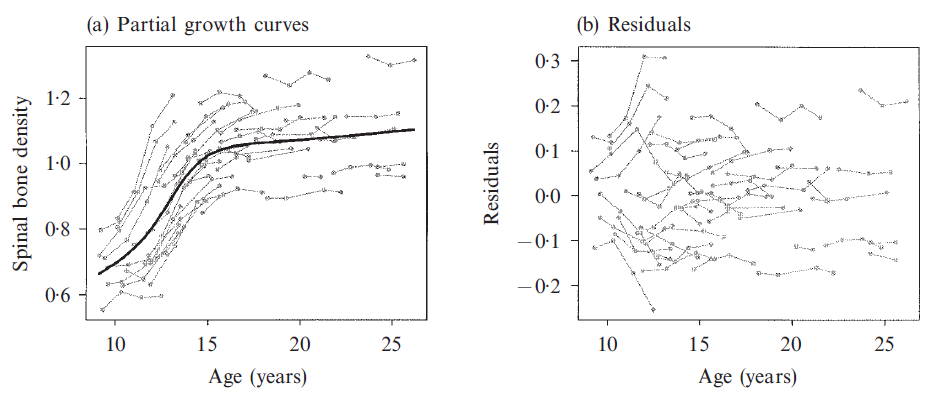
\includegraphics[width=0.7\linewidth]{img/1.png}
		\end{center}
		\label{fig:long}
		\label{fig:onecol}
	\end{figure}	
  \begin{itemize}
  	\item {
	    If each curves observed different time points, it is not good way to apply method with equal time points.
	}
	\item {
		In this paper, present an estimation technique when the data are sparse and measured at the different time points each curves.
	}	
  \end{itemize}
\end{frame}

\begin{frame}{Introduction}{A direct approach}
	\begin{block}{The direct method}
		When the curves are not measured at common time points, we estimate the curves by basis expansion and then perform PCA on the estimated curves.
	\end{block}
	\begin{block}{Drawbacks}
	\begin{itemize}
		\item {
			If each curves have few observation, there are not existed unique basis coefficients.
		}
		\item {
			The solution is not optimal ($\because$ perform PCA onto estimated curves)
		}
	\end{itemize}
	\end{block}
\end{frame}

\begin{frame}{Introduction}{A mixed effects approach}
	\begin{block}{Mixed effect model}
		$$ Y_i(t)=\mathbf{b}(t)^T\bbeta + \mathbf{b}(t)^T\bgamma_i+\epsilon_i(t), \ i=1,\dots,N $$
		where $\mathbf{b}(t)=[b_1(t),\dots,b_q(t)]^T $ is the vector of spline basis functions,
		$\bbeta$ is a fixed vector of spline coefficients, 
		$\bgamma_i$ is a random vector of spline coefficients with covariance matrix $\bGamma$, 
		$$ \bY_i=\bB_i\bbeta + \bB_i\bgamma_i + \bepsilon_i $$
		where $\bY_i$ is the $n_i$-dimensional vector, $\bB$ is the $n_i \times q$ spline basis matrix
	\end{block}
\end{frame}

\begin{frame}{Introduction}{A mixed effects approach}
	\begin{block}{Fitting the mixed effect model}
		\begin{itemize}
			\item {
				\texttt{EM} algorithm is used to fit the mixed effect model to estimate $\bbeta$ and $\bGamma$.
			}
			\item {
				Given these estimates $\bbeta$ and $\bGamma$, predictions are obtained  for the $\bgamma_i$'s using best linear unbiased prediction (BLUP)
				$$ \hat{\bgamma_i}= (\hat{\bGamma}^{-1}/\hat{\sigma}^2+\bB_i^T\bB_i)^{-1}\bB_i^T(\bY_i-\bB_i\hat{\bbeta}) $$
			}
			\item {
				Using the estimates of $\bbeta$ and $\bGamma$, we can estimate the mean and PC curves.
			}
			\item {
				Using the estimates of $\bbeta$ and $\bGamma$ and the prediction for $\bgamma_i$, we can predict the individual curve $\bY_i(t)$.
			}
		\end{itemize}
	\end{block}
	
\end{frame}

\begin{frame}{Introduction}{A mixed effects approach}
	\begin{block}{Advantages of the mixed effects model}
		\begin{itemize}
			\item {
				When the curve $Y_i(t)$ is insufficient, it can be used for estimating $Y_i(t)$ because of using all observation rather than $i$th curve.
			}
			\item {
				Using MLE to estimate $\bbeta, \bGamma$
			}
		\end{itemize}
	\end{block}
\end{frame}

\begin{frame}{Introduction}{Some problems with the mixed effects method}
	\begin{block}{Some problems with the mixed effects method}
		\begin{itemize}
			\item {
				The dimension of spline basis $=q$ \\
				$\Rightarrow$ \# of parameters of $\bGamma= \frac{q(q+1)}{2}$ 
			}
			\item {
				When the data are sparse, the estimate of $\bGamma$ is highly variable.\\
				$\Rightarrow$ \texttt{EM} algorithm converges to local maximum.
			}
		\end{itemize}
	\end{block}
\end{frame}

\begin{frame}{Introduction}{Some problems with the mixed effects method}
	\begin{figure}[h] %%% t: top, b: bottom, h: here
		\begin{center}
			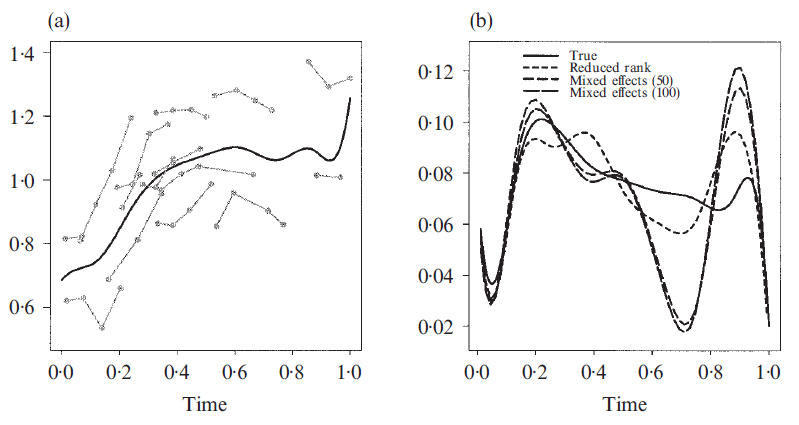
\includegraphics[width=0.7\linewidth]{img/2.png}
		\end{center}
		\label{fig:long}
		\label{fig:onecol}
	\end{figure}	
	\begin{itemize}
		\item {
			The direct method cannot be applied. ($\because n_i \ll q(=11)$)
		}
		\item {
			It looks overfitting in the mixed effect model.
		}
		\item {
			The reduced rank method presented in this paper looks better than the mixed effect method.
		}
	\end{itemize}
\end{frame}


\section{The Growth Curve Data}
\begin{frame}{The Growth Curve Data}
	\begin{multicols}{2}
		\begin{figure}[h] %%% t: top, b: bottom, h: here
			\begin{center}
				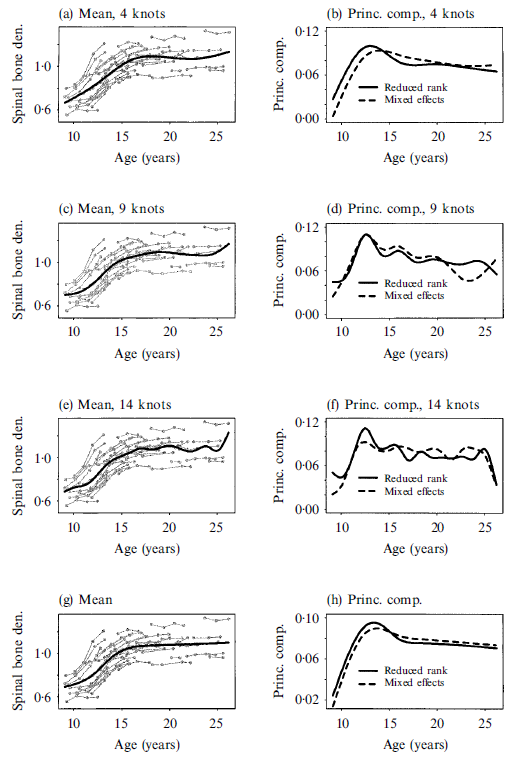
\includegraphics[width=1\linewidth]{img/3.png}
			\end{center}
			\label{fig:long}
			\label{fig:onecol}
		\end{figure}	
		\begin{itemize}
			\item {
				The curve is more wiggly as the \# of knots increases.
			}
			\item {
				In the reduced rank model, the peak is looked clear when $Age=13$.
			}
			\item {
				In the mixed effect model, the peak is not looked clear.
			}
		\end{itemize}
	\end{multicols}
\end{frame}


\section{The Reduced Rank Model}
\begin{frame}{The reduced rank model}
	\begin{block}{Generalized additive model}
		$$ Y_i(t)=\mu(t)+\sum_{j=1}^k f_j(t)\alpha_{ij}+\epsilon_i(t) = \mu(t)+\boldsymbol{f}(t)^T\balpha_i + \epsilon_i(t) $$
		subject to $\int f_jf_l=\delta_{jl}, \ the\ Kronecker \ \delta$, 
		$ \delta_{jl}=
		\begin{cases}
			1, & j=l \\
			0, & j \ne l
		\end{cases} $\\
		\vspace{0.3cm}
		where $\mu(t)$ is overall mean function, $f_j$ is the $j$th PC function, $\boldsymbol{f}=(f_1,\dots,f_k)^T$, $\balpha_i \sim (\mathbf{0},\Sigma)$, $\epsilon_i(t) \sim (\mathbf{0}, \sigma^2)$ and uncorrelated
	\end{block}

	In this paper, we let $\Sigma$ is diagonal.
\end{frame}

\begin{frame}{The reduced rank model}
	\begin{block}{Restrictions when data measured finite \# of time points}
		$$ \mu(t)=\mathbf{b}(t)^T\btheta_{\mu}, \ \ \boldsymbol{f}(t)^T=\mathbf{b}(t)^T\bTheta $$
		where $\mathbf{b}(t)$ is a spline basis with dimension $q$, $\bTheta$ is $q \times k$ spline coefficients matrix, $\btheta_{\mu}$ is $q$-dimensional vector of spline coefficients
	\end{block}
	\begin{block}{Restricted model}
		$$ Y_i(t)=\mathbf{b}(t)^T\btheta_{\mu}+\mathbf{b}(t)^T\bTheta\balpha_i + \epsilon_i(t) $$
		$$ \epsilon_i(t) \sim (\mathbf{0},\sigma^2), \ \balpha_i \sim (\mathbf{0}, \mathbf{D}) $$
		subject to
		$$ \bTheta^T \bTheta=\mathbf{I}, \ \int \mathbf{b}(t)^T\mathbf{b}(t)dt=1, \ \int\int \mathbf{b}(t)^T\mathbf{b}(s)dt=0 $$
		where $\mathbf{D}$ is diagonal.
	\end{block}	
\end{frame}

\begin{frame}{The reduced rank model}
	\begin{block}{Reduced rank model}
		$$ \bY_i=\mathbf{B}_i\btheta_{\mu}+\mathbf{B}_i\bTheta\balpha_i + \bepsilon_i $$
		$$ \bTheta^T \bTheta=\mathbf{I}, \ \bepsilon_i \sim (\mathbf{0}, \sigma^2 \mathbf{I}), \ \balpha_i \sim (\mathbf{0}, \mathbf{D}) $$
	\end{block}	
	\begin{itemize}
		\item {
			Parameters to estimate : $\btheta_{\mu}, \bTheta, \mathbf{D}, \sigma^2$
		}
		\item {
			mixed effect model + rank constraint on the covariance matrix (\# of PCs)
		}
	\end{itemize}
\end{frame}

\begin{frame}{The reduced rank model}{Mixed effect model}
	\begin{block}{Random vector with unrestricted covariance matrix}
		$$ \bgamma_i = [\bTheta, \bTheta^*]
						\begin{pmatrix}
							\balpha_i\\
							\balpha^*_i
						\end{pmatrix}
		$$
		where $\bgamma_i$ is $q$-dimensional vector in mixed effect model, $\bTheta^*$ is a $q \times (q-k)$ matrix, $\balpha_i$ is a random vector of length $q-k$ with diagonal covariance matrix.
	\end{block}	
	\begin{block}{Mixed effects model}
		$$ \bY_i=\mathbf{B}_i\btheta_{\mu}+\mathbf{B}_i\bTheta\balpha_i + \mathbf{B}_i\bTheta^*\balpha^*_i + \bepsilon_i $$
	\end{block}	
	\begin{itemize}
		\item {
			The ruduced rank model is a submodel of the mixed effects model.
		}
		\item {
			Set $\balpha^*_i=0$, it can be simply fitting the reduced rank model using a different algorithm.
		}
	\end{itemize}
\end{frame}

\begin{frame}{The reduced rank model}
	\begin{figure}[h] %%% t: top, b: bottom, h: here
		\begin{center}
			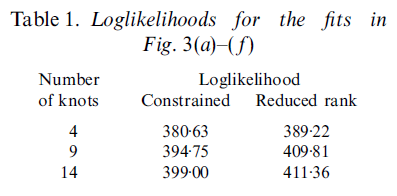
\includegraphics[width=0.7\linewidth]{img/4.png}
		\end{center}
		\label{fig:long}
		\label{fig:onecol}
	\end{figure}
	\begin{itemize}
		\item {
			The constrained mixed effects model obtained from the mixed effects model after setting the $\balpha^*_i=0$.
		}
		\item {
			The reduced rank likelihood is strictly higer than the constrained likelihood.
		}
	\end{itemize}
\end{frame}


\section{Fitting the Reduced Rank Model}
\begin{frame}{Fitting the Reduced Rank Model}{Preamble}
	\begin{block}{Goal of FPCA}
		\begin{itemize}
			\item {
				Estimate $\mu$ and $f$
			}
			\item {
				Prediction of the basis coefficients $\balpha_i$
			}
		\end{itemize}
	\end{block}
	Assuming the spline fit to the functions, it is equivalent to estimate $\btheta_{\mu}$, $\bTheta$ and predict the $\balpha_i$
	\begin{itemize}
		\item {
			Parameters to estimate : $\btheta_{\mu}, \bTheta, \sigma^2, \mathbf{D}$
		}
		\item {
			$\mathbf{D}$ : variability explained by each PC curve
		}
		\item {
			$\sigma^2$ : variability left unexplained
		}
	\end{itemize}
	\begin{block}{Two fitting procedures}
		\begin{itemize}
			\item {
				Maximum likelihood
			}
			\item {
				Penalized least squares
			}
		\end{itemize}
	\end{block}
\end{frame}

\begin{frame}{Fitting the Reduced Rank Model}{Maximum likelihood}
	Assume that $\bepsilon_i \sim N(\mathbf{0},\sigma^2 \mathbf{I})$ and $\balpha_i \sim N(\mathbf{0}, \mathbf{D})$.
	$$ \bY_i \sim N(\mathbf{B}_i\btheta_{\mu}, \sigma^2\mathbf{I}+\mathbf{B}_i\bTheta\mathbf{D}\bTheta^T\mathbf{B}^T_i) $$
	The observed likelihood of the $\bY_i$'s is
	$$ \prod_{i=1}^N \frac{1}{(2\pi)^{n_i/2}|\sigma^2\mathbf{I}+\mathbf{B}_i\bTheta\mathbf{D}\bTheta^T\mathbf{B}^T_i|^{1/2}} $$
	$$ \times \exp \bigg \{ -\frac{1}{2}(\bY_i-\mathbf{B}_i\btheta_{\mu})^T(\sigma^2\mathbf{I}+\mathbf{B}_i\bTheta\mathbf{D}\bTheta^T\mathbf{B}^T_i)^{-1} (\bY_i-\mathbf{B}_i\btheta_{\mu}) \bigg \} $$
	\begin{itemize}
		\item {
			But to maximize this likelihood is a nonconvex optimization problem.
		}
	\end{itemize}	
\end{frame}

\begin{frame}{Fitting the Reduced Rank Model}{Maximum likelihood}
	If $\balpha_i$'s were observed, the joint likelihood is simplified to
	$$ \prod_{i=1}^N \frac{1}{(2\pi)^{(n_i+k)/2}\sigma^{n_i}|\mathbf{D}|^\frac{1}{2}} $$
	$$ \times \exp \bigg \{ -\frac{1}{2\sigma^2}(\bY_i-\mathbf{B}_i\btheta_{\mu}-\mathbf{B}_i\bTheta\balpha_i)^T(\bY_i-\mathbf{B}_i\btheta_{\mu}-\mathbf{B}_i\bTheta\balpha_i) - \frac{1}{2}\balpha_i^T\mathbf{D}^{-1}\balpha_i \bigg \} $$
	
	\begin{itemize}
		\item {
			Let $\balpha_i$ is unobserved(missing), we can maximize this likelihood much easier using \texttt{EM} algorithm.
		}
	\end{itemize}	
\end{frame}

\begin{frame}{Fitting the Reduced Rank Model}{Penalized least squares}
	We choose $\btheta_{\mu}, \bTheta, \balpha_i$'s to minimize the sum of squared residuals,
	$$ \sum_{i=1}^N \bigg \{ (\bY_i-\mathbf{B}_i\btheta_{\mu}-\mathbf{B}_i\bTheta\balpha_i)^T(\bY_i-\mathbf{B}_i\btheta_{\mu}-\mathbf{B}_i\bTheta\balpha_i) + \sigma^2 \sum_{j=1}^K \frac{\alpha^2_{ij}}{\mathbf{D}_{jj}} \bigg \} $$
	
	\begin{itemize}
		\item {
			Minimize SSE $\Leftrightarrow$ Maximize likelihood
		}
		\item {
			Distribution assumption X
		}
		\item {
			It can be maximized using \texttt{EM} algorithm.
		}	
	\end{itemize}	
\end{frame}


\section{The Reduced Rank and Mixed Effects Methods Compared}
\begin{frame}{The Reduced Rank and Mixed Effects Methods Compared}
	\begin{block}{Study 1}
		\begin{itemize}
			\item {
				Generate data from the mean function and PC curve corresponding to reduced rank fit using spline with knots at ages 12, 14, 16 and 18.
			}
			\item {
				48 curves were generated using same time points as the growth curve data.
			}
		\end{itemize}
	\end{block}
	\begin{block}{Study 2}
		\begin{itemize}
			\item {
				Generate data in the same way as study 1 except that using spline with 7 equally spaced knots were used.
			}
			\item {
				16 curves were generated using randomly selected time points of the original 48 growth curves.
			}
		\end{itemize}
	\end{block}
	In two studies, mixed effects and reduced rank model were fitted to 10 datasets using natural cubic splines.
\end{frame}

\begin{frame}{The Reduced Rank and Mixed Effects Methods Compared}
	\begin{block}{Study 1}
		\begin{figure}[h] %%% t: top, b: bottom, h: here
			\begin{center}
				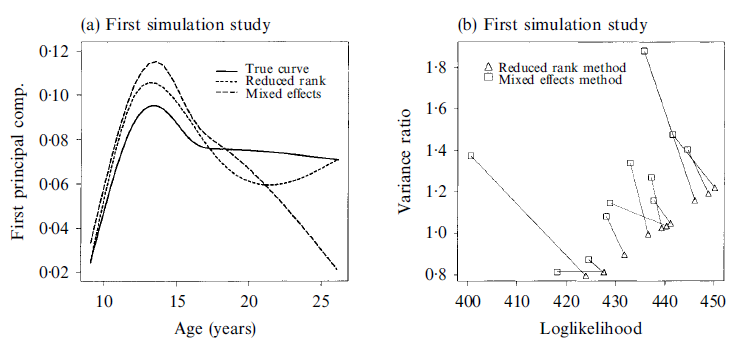
\includegraphics[width=0.7\linewidth]{img/5.png}
			\end{center}
			\label{fig:long}
			\label{fig:onecol}
		\end{figure}
		\begin{itemize}
			\item {
				In Figure (a), the reduced rank fit looks better than the mixed effects fit.
			}
			\item {
				In Figure (b),\\
				almost all the variance ratios for mixed effects fits $> 1$\\
				$\Rightarrow$ mixed effects fit underestimates the variance.(overfitting)
			}
			\item {
				Reduced rank fits have higher likelihood on all 10 datasets.
			}
		\end{itemize}
	\end{block}
\end{frame}

\begin{frame}{The Reduced Rank and Mixed Effects Methods Compared}
	\begin{block}{Study 2}
		\begin{figure}[h] %%% t: top, b: bottom, h: here
			\begin{center}
				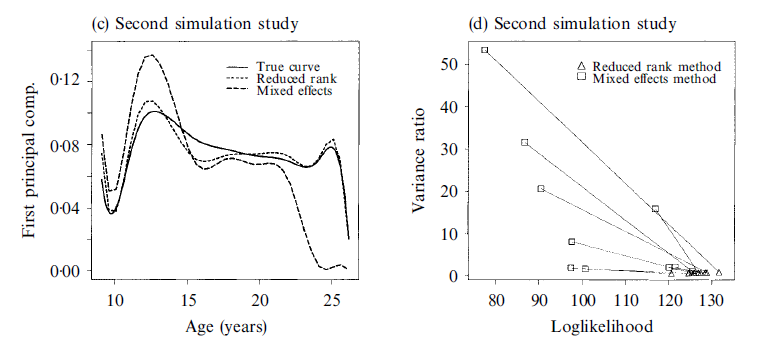
\includegraphics[width=0.7\linewidth]{img/6.png}
			\end{center}
			\label{fig:long}
			\label{fig:onecol}
		\end{figure}
		\begin{itemize}
			\item {
				In Figure (c), the reduced rank fit looks better than the mixed effects fit.
			}
			\item {
				In Figure (d), overfitting has increased on mixed effects fit.
			}
			\item {
				The likelihood estmate becomes worse as the variance is underestimated.
			}
		\end{itemize}
	\end{block}
\end{frame}


\section{Model Selection and Inference}
\begin{frame}{Model Selection and Inference}{Selection of the number of knots in the spline basis}
	Select the number using cross validation to maximize the loglikelihood for different numbers of knots.
	\begin{figure}[h] %%% t: top, b: bottom, h: here
		\begin{center}
			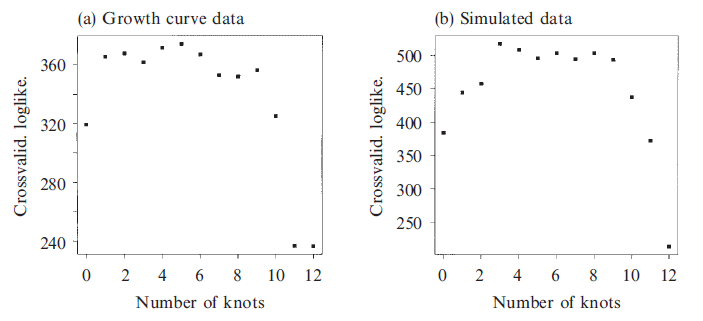
\includegraphics[width=0.7\linewidth]{img/7.png}
		\end{center}
		\label{fig:long}ㅡ
		\label{fig:onecol}
	\end{figure}
	\begin{itemize}
		\item {
			In Figure (a), the optimal number of knots is between 4 and 6, we opted 4 knots for the law of parsimony.
		}
		\item {
			In Figure (b), data simulated from a spline with 4 knots but likelihood is maximized for 3 knots.
		}
	\end{itemize}
\end{frame}

\begin{frame}{Model Selection and Inference}{Selection of the rank, $k$}
	Selecting the rank of the covariance matrix $=$ Selecting \# of PCs
	\begin{block}{Methods to select the rank, $k$}
		\begin{itemize}
			\item {
				PVE (Proportion of Variance Explained)
			}
			\item {
				Comparison loglikelihood with different $k$
			}
		\end{itemize}
	\end{block}
\end{frame}

\begin{frame}{Model Selection and Inference}{Selection of the rank, $k$}
	\begin{block}{PVE}
		\begin{itemize}
			\item {
				PVE is difficult to compute directly in FPCA.
			}
			\item {
				If $\sigma^2 \rightarrow 0$ and all curves are measured at similar time points, $Var(\bY_i) \approx Var(\balpha_i) = \mathbf{D}$
			}
			\item {
				PVE $= \frac{\mathbf{D}_{jj}}{tr(\mathbf{D})}, \ (\because \ \mathbf{D} $ is diagonal)
			}
		\end{itemize}
	\end{block}
\end{frame}

\begin{frame}{Model Selection and Inference}{Selection of the rank, $k$}
	\begin{figure}[h] %%% t: top, b: bottom, h: here
		\begin{center}
			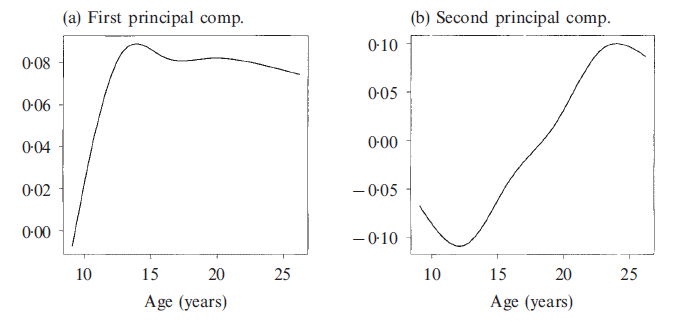
\includegraphics[width=0.7\linewidth]{img/8.png}
		\end{center}
		\label{fig:long}
		\label{fig:onecol}
	\end{figure}
	\begin{itemize}
		\item {
			In 1st PC, a sharp peak indicates the puberty periods which shows the highest variability with each curves. 
		}
		\item {
			2nd PC indicates differences in the slopes of individual curves. If the weight of PC2 increases, this curve has slope greater than average.
		}
	\end{itemize}
\end{frame}

\begin{frame}{Model Selection and Inference}{Selection of the rank, $k$}
	\begin{block}{Comparison loglikelihood with different $k$}
		\begin{itemize}
			\item {
				The loglikelihood increases as $k$ increases.
			}
			\item {
				Pick the $k$ when the increase levelled off.
			}
			\item {
				Example of graphical selection
			}
		\end{itemize}
		\begin{figure}[h] %%% t: top, b: bottom, h: here
			\begin{center}
				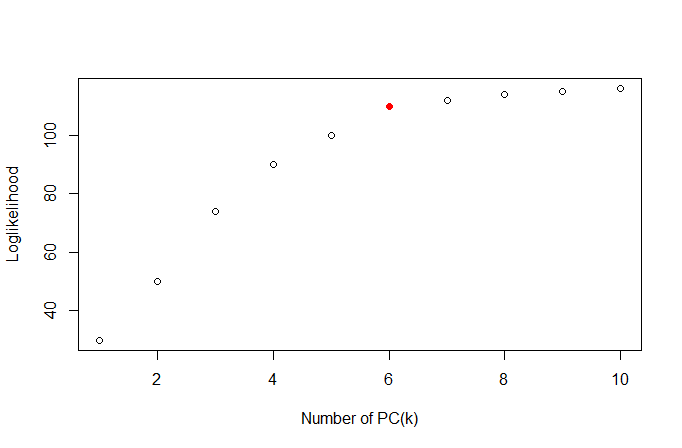
\includegraphics[width=0.6\linewidth]{img/9.png}
			\end{center}
			\label{fig:long}
			\label{fig:onecol}
		\end{figure}
	\end{block}
\end{frame}

\begin{frame}{Model Selection and Inference}{Selection of the rank, $k$}
	\begin{block}{Comparison loglikelihood with different $k$}
		\begin{itemize}
			\item {
				LRT test
			}
			\begin{itemize}
				\item {
					$H_0:k=k_0$ vs $H_1:k=k_1$
				}
				\item {
					$LRT = 2(\log L_{k=k_1} - \log L_{k=k_0}) \ \dot\sim \ \chi^2_{df}$, \\where $df=$ difference of parameters
				}
			\end{itemize}
			\item {
				Example
			}
			\begin{itemize}
				\item {
					$H_0:k=1$ vs $H_1:k=2$
				}
				\item {
					$LRT = 2(\log L_{k=2} - \log L_{k=1}) = 19.28 \ \dot\sim \ \chi^2_5$,\\
					$p$-value $=0.002$
				}
				\item {
					Reject $H_0$, we choose $k=2$.
				}
				\item {
					But this dataset is sparse, we shoud caution when using an asymptotic result
				}
			\end{itemize}
		\end{itemize}
	\end{block}\
\end{frame}

\begin{frame}{Model Selection and Inference}{Confidence intervals}
	To compute confidence intervals for the overall mean function, PCs and individual curves, we use the bootstrap.
	\begin{block}{Two methods to bootstrap curve data}
		\begin{itemize}
			\item {
				Resampling the individual curves.
			}
			\begin{itemize}
				\item {
					No parametric assumption
				}
				\item {
					Sparse data $\Rightarrow$ performance $\downarrow$
				}
			\end{itemize}
			\item {
				Resampling the estimated $\balpha_i$'s and residuals and generating new partial curves based on these values.
			}
			\begin{itemize}
				\item {
					Bootstrap datasets have observations at the same time points as the original dataset.
				}
			\end{itemize}
		\end{itemize}
	\end{block}
\end{frame}

\begin{frame}{Model Selection and Inference}{Confidence intervals}
	\begin{block}{Confidence intervals on the growth curve data}
		\begin{itemize}
			\item {
				Generate $100$ bootstrap samples and fit the reduced rank method with $k=2$ to each
			}
			\item {
				Using the bootstrap percentile method, we computed $80\% \text{ and } 90\%$ CIs.
			}
		\end{itemize}
	\end{block}
\end{frame}

\begin{frame}{Model Selection and Inference}{Confidence intervals}
	\begin{figure}[h] %%% t: top, b: bottom, h: here
		\begin{center}
			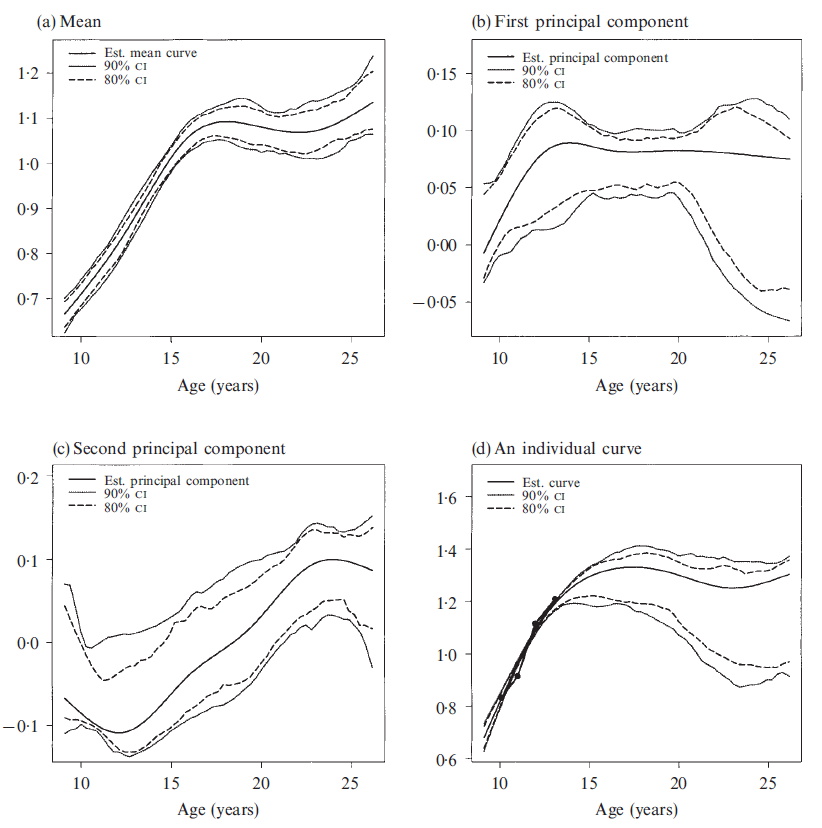
\includegraphics[width=0.6\linewidth]{img/10.png}
		\end{center}
		\label{fig:long}
		\label{fig:onecol}
	\end{figure}
\end{frame}


\section{Comparison of the Reduced Rank Method and Classical Principal Components}
\begin{frame}{Comparison of the Reduced Rank Method and Classical Principal Components}
	The linear model
	$$ \bX_i = \btheta_{\mu}+\bTheta\balpha_i + \bepsilon_i $$
	$$ \bepsilon_i \sim N(\mathbf{0}, \mathbf{\Sigma}), \ \balpha_i \sim N(\mathbf{0},\mathbf{D}) $$
	where $\bX_i$ are $q$-dimensional data vectors, $\bTheta$ is an orthogonal matrix
	\begin{itemize}
		\item {
			$\mathbf{\Sigma}$ is diagonal $\Rightarrow$ MLE of linear model is equivalent to factor analysis solution.
		}
		\item {
			$\mathbf{\Sigma}=\sigma^2 \mathbf{I}$ $\Rightarrow$ if $\sigma^2 \rightarrow 0$, then MLE of linear model is equivalent to classical PCA solution with minimizing
			$$ \sum_{i=1}^N \Vert \bX_i - \btheta_{\mu}-\bTheta\balpha_i \Vert^2  $$
		}
	\end{itemize}
\end{frame}

\begin{frame}{Comparison of the Reduced Rank Method and Classical Principal Components}
	The reduced rank model
	$$ \bY_i = \mathbf{B}_i\btheta_{\mu}+\mathbf{B}_i\bTheta\balpha_i + \bepsilon_i, \ Cov(\bepsilon_i)=\sigma^2\mathbf{I} $$
	where $\bTheta$ is the PCs and the $\balpha_i$'s are weights for the PC
	\begin{itemize}
		\item {
			$Cov(\bepsilon_i)=\sigma^2 \mathbf{I}$ $\Rightarrow$ Solution of reduced rank model is equivalent to generalized PCA solution.
		}
		\item {
			On penalized least squares objective function,\\ if $\sigma^2 \rightarrow 0$, then the procedure for fitting the reduced rank model simply minimizes
		$$ \sum_{i=1}^N \Vert \bY_i - \mathbf{B}_i\btheta_{\mu} - \mathbf{B}_i\bTheta\balpha_i \Vert^2  $$
		}
	\end{itemize}
\end{frame}

\begin{frame}{Comparison of the Reduced Rank Method and Classical Principal Components}
	Let $\hat{\bgamma_i}=(\mathbf{B}^T_i\mathbf{B}_i)^{-1}\mathbf{B}^T_i\bY_i$, LSE of the spline coefficients for $i$th curve, then objective equation is
	$$ \sum_{i=1}^N \Vert \bY_i - \mathbf{B}_i\hat{\bgamma_i} \Vert^2 + \sum_{i=1}^N \Vert \mathbf{B}_i\hat{\bgamma_i} - \mathbf{B}_i\btheta_{\mu} - \mathbf{B}_i\bTheta\balpha_i \Vert^2  $$
	$$ = C(\bY) + \sum_{i=1}^N \Vert \hat{\bgamma_i} - \btheta_{\mu} - \bTheta\balpha_i \Vert_{\mathbf{B}^T_i\mathbf{B}_i}^2 $$
	where $C(\bY)$ is a constant with the parameters.\\
	Therefore, we minimize
	$$ \sum_{i=1}^N \Vert \hat{\bgamma_i} - \btheta_{\mu} - \bTheta\balpha_i \Vert_{\mathbf{B}^T_i\mathbf{B}_i}^2 $$
\end{frame}

\begin{frame}{Comparison of the Reduced Rank Method and Classical Principal Components}
	\begin{itemize}
		\item {
			If all curves are measured at the same time points, then $\mathbf{B}_i=\mathbf{B}$.
		}
		\item {
			WLOG, assume $\mathbf{B'B=I}$, minimizing the objective equation is equivalent to performing standard PCA on the spline coefficients. $\Rightarrow$ the direct method
		}
		\item {
			Similarly to classical PCA, When all curves are measured at the same time points, the reduced rank method finds the best plane using the Euclidean metric.
		}
		\item {
			Also it finds the best plane when the curves are not measured at the same time points, but the distance between the plane and each data point is measured relative to the metric $\bB_i^T\bB_i$.
		}
	\end{itemize}
\end{frame}


\section{Appendix}
\begin{frame}{Appendix}{BLUP(Best Linear Unbiased Prediction)}
	The mixed model
	$$\by = \bX \bbeta+\bZ\bu+\bepsilon$$
	$$\bu \sim (\mathbf{0},\bG), \ \bepsilon \sim (\mathbf{0},\bR), \ Var(\by)=\bV=\bZ\bG\bZ^T+\bR, \ Cov(\bu,\bepsilon)=\mathbf{0} $$
	Assume $\by|\bu \sim N(\bX \bbeta+\bZ\bu,\bR)$ and $\bu \sim N(\mathbf{0},\bG)$,\\
	then likelihood function is
	$$ -2\log f(\by|\bu)=N\log 2\pi+\log|\bR|+(\by-\bX  \bbeta-\bZ\bu)^T\bR^{-1}(\by-\bX \bbeta-\bZ\bu) $$
	$$ -2\log f(\bu)= q\log 2\pi + \log|\bG| + \bu^T\bG^{-1}\bu $$
	Maximizing $l(\bbeta,\bu|\by)=\log f(\by,\bu)$ is equivalent to minimizing the sum of the two equations.
\end{frame}

\begin{frame}{Appendix}{BLUP(Best Linear Unbiased Prediction)}
	Differentiating the sum of the two equations
	$$ \begin{aligned}
	\frac{\partial [-2l(\bbeta,\bu|\by)]}{\partial \bbeta} &= -2\bX^T\bR^{-1}(\by-\bX\bbeta-\bZ\bu)\\
	\frac{\partial [-2l(\bbeta,\bu|\by)]}{\partial \bu} &= -2\bZ^T\bR^{-1}(\by-\bX\bbeta-\bZ\bu)+2\bG^{-1}\bu
	\end{aligned} $$ 
	equating them to $0$ gives the following system 
	$$ \bX^T\bR^{-1}\bX\hat{\bbeta}+\bX^T\bR^{-1}\bZ\hat{\bu}=\bX^T\bR^{-1}\by $$
	$$ \bZ^T\bR^{-1}\bX\hat{\bbeta}+(\bZ^T\bR^{-1}\bZ+\bG^{-1})\hat{\bu}=\bZ^T\bR^{-1}\by $$
	called Henderson's mixed model equations (HMME)
\end{frame}

\begin{frame}{Appendix}{BLUP(Best Linear Unbiased Prediction)}
	The matrix form of HMME is
	$$ \begin{pmatrix}
		\bX^T\bR^{-1}\bX & \bX^T\bR^{-1}\bZ \\
		\bZ^T\bR^{-1}\bX& \bZ^T\bR^{-1}\bZ+\bG^{-1}
	\end{pmatrix}
	\begin{pmatrix}
	\hat{\bbeta} \\
	\hat{\bu}
	\end{pmatrix} =
	\begin{pmatrix}
	\bX^T\bR^{-1}\by \\
	\bZ^T\bR^{-1}\by
	\end{pmatrix} $$
	Solve this equation,
	$$
	\begin{aligned}
	\hat{\bbeta} &= (\bX^T\bV^{-1}\bX)^{-1}\bX^T\bV^{-1}\by = \hat{\bbeta}^{GLS}\\
	\hat{\bu} &= (\bZ^T\bR^{-1}\bZ+\bG^{-1})^{-1}\bZ^T\bR^{-1}(\by-\bX\hat{\bbeta})
	\end{aligned}$$
	where $\hat{\bbeta}$ is BLUE(Best Linear Unbiased Estimator) and $\hat{\bu}$ is BLUP(Best Linear Unbiased Prediction)
\end{frame}

\appendix
\section{Reference}
\begin{frame}
  \frametitle<presentation>{Reference}
    
  \begin{thebibliography}{10}
  	\beamertemplatearticlebibitems
	% Followed by interesting articles. Keep the list short. 
	\bibitem{Someone2000}
	GARETH M. JAMES, TREVOR J. HASTIE, CATHERINE A. SUGAR
	\newblock Principal component models for sparse functional data
	\newblock {\em Biometrika}, 87(3):587--602,
	2000.
    
  \beamertemplatebookbibitems
  % Start with overview books.
	\bibitem{Author1990}
		J.O. Ramsay, B.W. Silverman.
		\newblock {\em Functional Data Analysis 2nd edition}.
		\newblock Springer, 2005.

  \end{thebibliography}
\end{frame}


% All of the following is optional and typically not needed. 
%\appendix
%\section<presentation>*{\appendixname}
%\subsection<presentation>*{For Further Reading}
%
%\begin{frame}[allowframebreaks]
%  \frametitle<presentation>{For Further Reading}
%    
%  \begin{thebibliography}{10}
%    
%  \beamertemplatebookbibitems
%  % Start with overview books.
%
%  \bibitem{Author1990}
%    A.~Author.
%    \newblock {\em Handbook of Everything}.
%    \newblock Some Press, 1990.
% 
%    
%  \beamertemplatearticlebibitems
%  % Followed by interesting articles. Keep the list short. 
%
%  \bibitem{Someone2000}
%    S.~Someone.
%    \newblock On this and that.
%    \newblock {\em Journal of This and That}, 2(1):50--100,
%    2000.
%  \end{thebibliography}
%\end{frame}

\end{document}


